\documentclass[12pt,a4paper]{amsart}
\usepackage{amssymb}
\usepackage[a4paper,left=2.25cm,right=2.25cm,top=3cm,bottom=3cm,headsep=1cm]{geometry}
\usepackage{tikz}%\usetikzlibrary{fit,positioning,matrix,calc,decorations.markings,angles,decorations.pathmorphing,decorations.pathreplacing}%,matrix,fit,shapes.geometric}
\title{Example file for M2inTeX}
\author{Paul Zinn-Justin}
\begin{document}
\maketitle

\section{Introduction}
some basic examples:
% start M2
\begin{verbatim}
i1 : R=QQ[x,y]; factor(x^3-y^3)
\end{verbatim}
\noindent\verb|o2 = |$\left(x-y\right)\left(x^{  2}+x\,y+y^{  2}\right)$

\noindent\verb|o2 : |$\texttt{Expression}\texttt{ of class }\texttt{Product}$
% start M2
\begin{verbatim}
i3 : res coker vars R
\end{verbatim}
\noindent\verb|o3 = |$\underset{\vphantom{\Big|}0}{R^{  1}}\,\xleftarrow{\left(\begin{smallmatrix}
x&y\\
\end{smallmatrix}\right)}\,\underset{\vphantom{\Big|}1}{R^{  2}}\,\xleftarrow{\left(\begin{smallmatrix}
-y\\
x\\
\end{smallmatrix}\right)}\,\underset{\vphantom{\Big|}2}{R^{  1}}\,\xleftarrow{0}\,\underset{\vphantom{\Big|}3}{0}$

\noindent\verb|o3 : |$\texttt{ChainComplex}$

more:
% start M2
\begin{verbatim}
i4 : 318/46
\end{verbatim}
\noindent\verb|o4 = |$\frac{159}{ 23}$

\noindent\verb|o4 : |${\mathbb Q}$
% start M2
\begin{verbatim}
i5 : exp 3.73767
\end{verbatim}
\noindent\verb|o5 = |${42}$

\noindent\verb|o5 : |${\mathbb R}\texttt{ (of precision } 53\texttt{)}$

strings:
% start M2
\begin{verbatim}
i6 : "hehe"
\end{verbatim}
\noindent\verb|o6 = |hehe

and nets: TODO fix {\tt tex Net}
% start M2
\begin{verbatim}
i7 : "haha"||"hihi"
\end{verbatim}
\noindent\verb|o7 = |$\begin{array}{l}\texttt{haha}\\
\texttt{hihi}\end{array}$


\section{Help}
% start M2
\begin{verbatim}
i8 : help det
\end{verbatim}
\noindent\verb|o8 = |
\par \medskip\noindent\begingroup\Large\bf
determinant -- determinant of a matrix\endgroup
\par \smallskip%

\par \medskip\noindent\begingroup\Large\bf
Synopsis\endgroup
\par \smallskip%
\begin{itemize}
\item 
\par Usage: 
\par \begingroup\tt det\ M\endgroup{}
\item Inputs:\begin{itemize}
\item \begingroup\tt M\endgroup{}, a square \begingroup\tt matrix\endgroup{}
\end{itemize}

\item \begingroup\tt Optional\ inputs\endgroup{}:\begin{itemize}
\item \begingroup\tt Strategy\endgroup{}\begingroup\tt \ ={\char 62}\ \endgroup{}\begingroup\tt ...\endgroup{}, default value null, choose between Bareiss and Cofactor algorithms
\end{itemize}

\item Outputs:\begin{itemize}
\item a \begingroup\tt ring\ element\endgroup{}, which is the determinant of \begingroup\tt M\endgroup{}
\end{itemize}

\end{itemize}

\par \medskip\noindent\begingroup\Large\bf
Description\endgroup
\par \smallskip%

\par \medskip\noindent\begingroup\Large\bf
See also\endgroup
\par \smallskip%
\begin{itemize}
\item \begingroup\tt exteriorPower\endgroup{} -- exterior power
\item \begingroup\tt minors\endgroup{} -- ideal generated by minors
\item \begingroup\tt permanents\endgroup{} -- ideal generated by square permanents of a matrix
\item \begingroup\tt pfaffians\endgroup{} -- ideal generated by Pfaffians
\end{itemize}

\par \medskip\noindent\begingroup\Large\bf
Ways to use \begingroup\tt determinant\endgroup{} :\endgroup
\par \smallskip%
\begin{itemize}
\item \begingroup\tt {\char 34}determinant(Matrix){\char 34}\endgroup{}
\item \begingroup\tt {\char 34}determinant(MutableMatrix){\char 34}\endgroup{}
\end{itemize}

\par \medskip\noindent\begingroup\Large\bf
For the programmer\endgroup
\par \smallskip%

\par The object \begingroup\tt determinant\endgroup{} is a \begingroup\tt method\ function\ with\ options\endgroup{}.

\noindent\verb|o8 : |$\texttt{DIV}$


\section{packages}
packages that have a {\tt tex} output will work:
% start M2
\begin{verbatim}
i9 : needsPackage "Posets";
\end{verbatim}
% start M2
\begin{verbatim}
i10 : booleanLattice 3
\end{verbatim}
\noindent\verb|o10 = |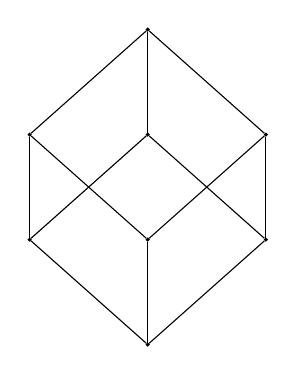
\begin{tikzpicture}[scale=1, vertices/.style={draw, fill=black, circle, inner sep=0pt}]
	\node [vertices] (0) at (-0+0,0){};
	\node [vertices] (1) at (-1.5+0,1.33333){};
	\node [vertices] (2) at (-1.5+1.5,1.33333){};
	\node [vertices] (4) at (-1.5+3,1.33333){};
	\node [vertices] (3) at (-1.5+0,2.66667){};
	\node [vertices] (5) at (-1.5+1.5,2.66667){};
	\node [vertices] (6) at (-1.5+3,2.66667){};
	\node [vertices] (7) at (-0+0,4){};
\foreach \to/\from in {0/1, 2/3, 0/2, 1/3, 4/5, 6/7, 4/6, 5/7, 0/4, 1/5, 2/6, 3/7}
\draw [-] (\to)--(\from);
\end{tikzpicture}


\noindent\verb|o10 : |$\texttt{Poset}$


\section{multi-line example}
% start M2
\begin{verbatim}
i11 : f = i -> (
      i+1
      )
\end{verbatim}
\noindent\verb|o11 = |$\texttt{f}$

\noindent\verb|o11 : |$\texttt{FunctionClosure}$



\end{document}
